\section{Results and Analyses}

\begin{figure*}[t]
    \centering
    
\includegraphics[width=0.92\linewidth]{Figure_srcs/shared_legend.pdf}
    \\[-0.02in]
    \begin{minipage}[t]{0.62\linewidth}
        \centering
        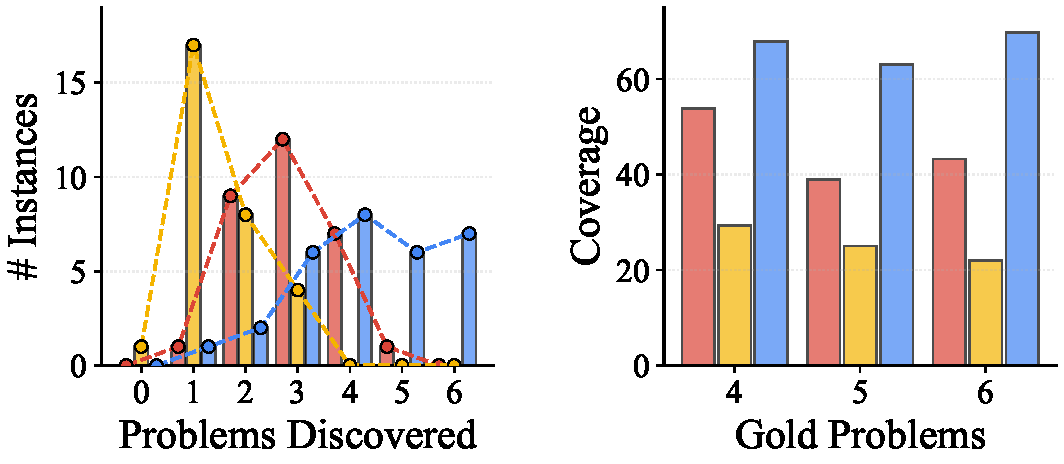
\includegraphics[width=0.975\linewidth]{Figure_srcs/multi_bottleneck_scaling.pdf}
        \vspace{-0.075in}
        \captionof{figure}{Multi-problem discovery on the Workspace setting with GPT. Left: discovered problems per instance. Right: coverage by gold count.}
        \label{fig:multi_bottleneck_scaling}
    \end{minipage}\hfill
    \begin{minipage}[t]{0.36\linewidth}
        \centering
        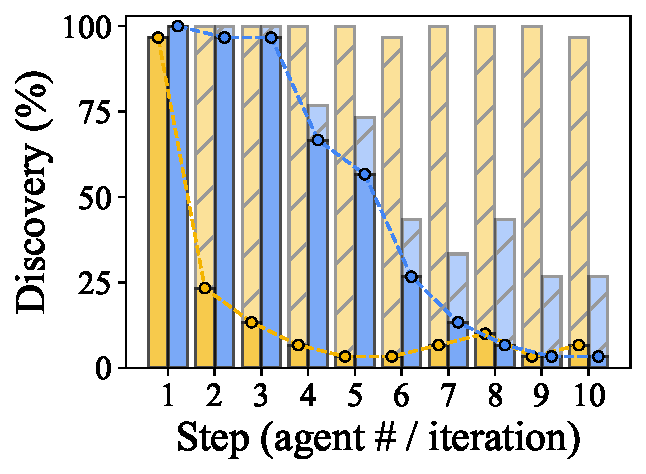
\includegraphics[width=0.975\linewidth]{Figure_srcs/multi_agent_vs_tide_diversity.pdf}
        \vspace{-0.075in}
        \captionof{figure}{Newly vs.\ re-discovered predictions on the Workspace task with GPT.}
        \label{fig:diversity}
    \end{minipage}
\end{figure*}


\subsection{Main Results}
Table~\ref{tab:main} shows performance on retrieval, identification, and resolution across the Workspace and Repository settings, under four LLM backbones.
Although recent LLMs can process the entire candidate pool in a single long-context pass, this access alone is insufficient for multi-problem discovery.
This is reflected in the \textsc{Single-Agent} baseline, which commits to its first hypotheses without revisiting the context and leaves the majority of gold problems undiscovered.
Surprisingly, running the same backbone as multiple independent agents in parallel does not close this gap.
In contrast, \textsc{TIDE} combines iterative discovery with reusable templates, consistently achieving the best performance across retrieval, identification, and resolution.

\subsection{In-Depth Analyses}

\paragraph{Discovery on Multi-Problem Instances.}
Our framework targets multi-problem instances, where recovering a single problem is not enough.
To directly assess this capability, we report results in Figure~\ref{fig:multi_bottleneck_scaling}, where every instance contains four to six gold problems.
Both baselines mostly discover only one or two problems per instance (left), while \textsc{TIDE} often reaches four or more.
Moreover, across instances with increasing numbers of gold problems (right), \textsc{TIDE} consistently continues to recover most of them while the baselines lag further behind, with \textsc{Multi-Agent} even falling below the simpler \textsc{Single-Agent}.

\begin{figure}[!t]
    \centering
    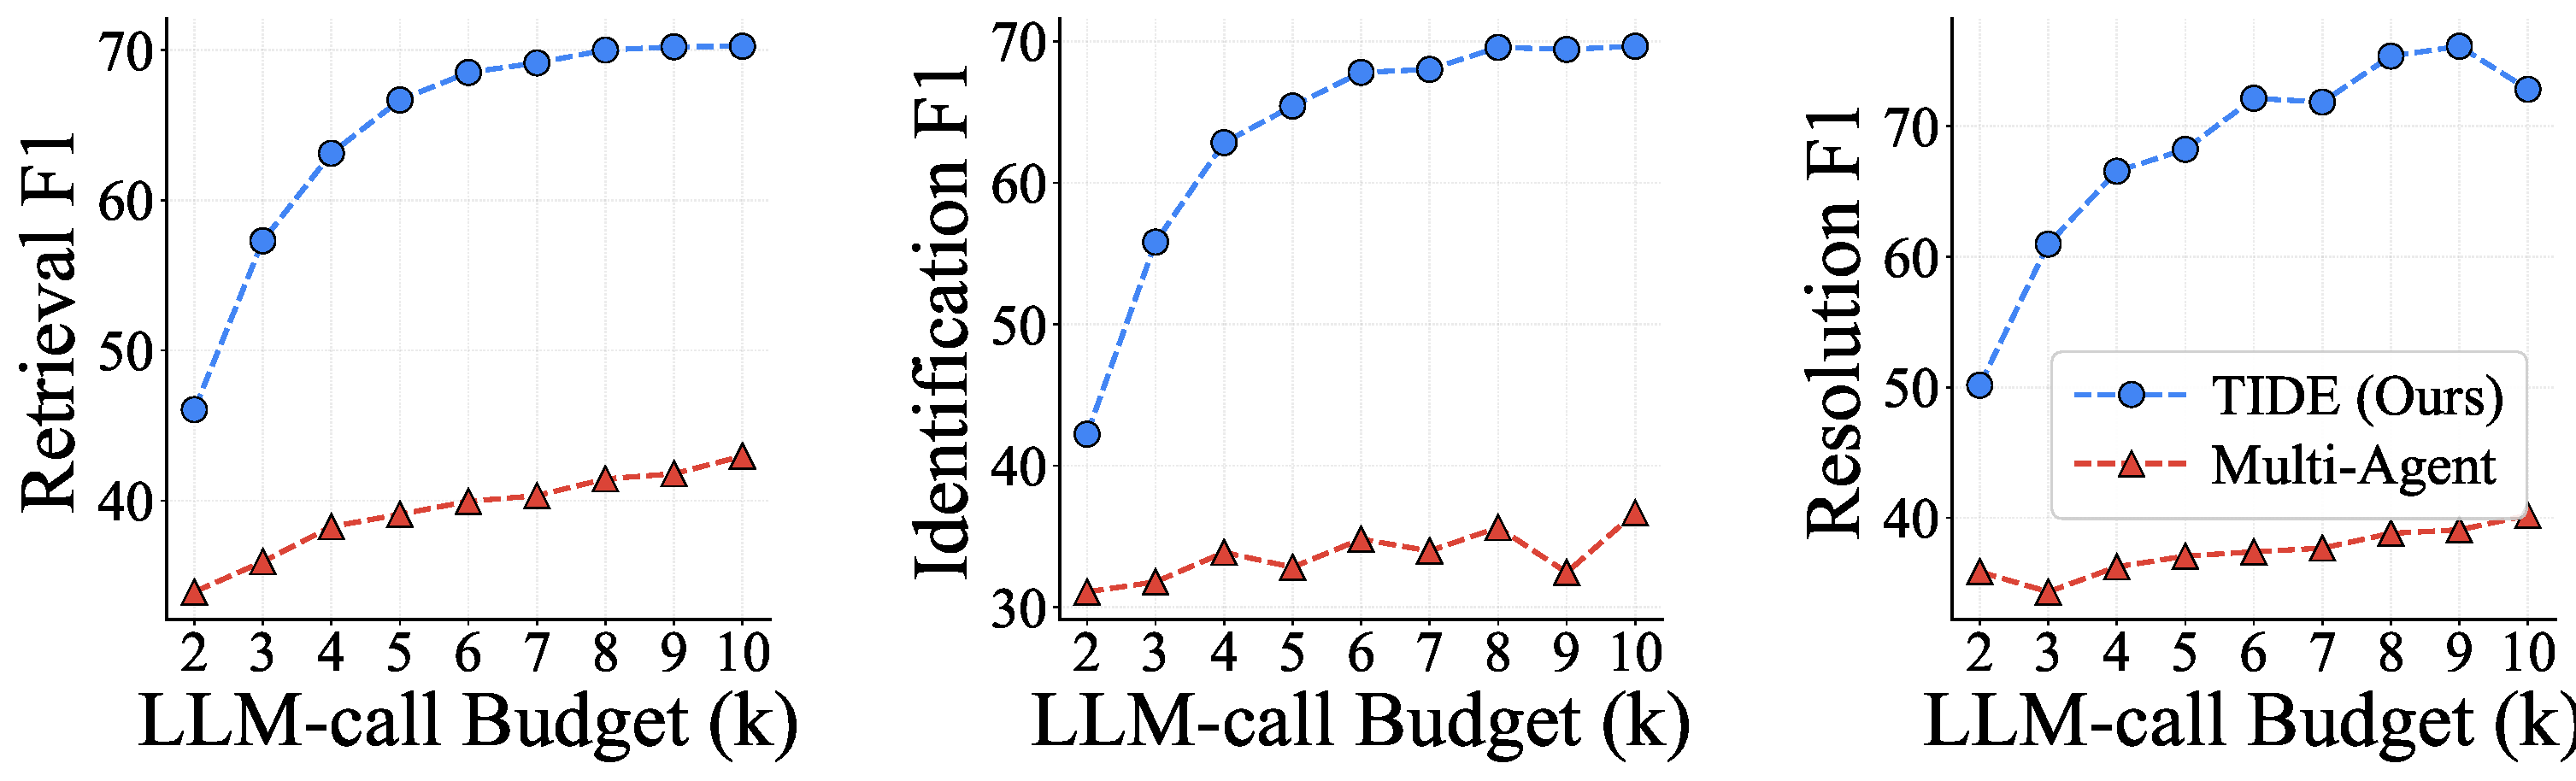
\includegraphics[width=0.975\linewidth]{Figure_srcs/budget_scaling.pdf}
    \vspace{-0.075in}
    \caption{F1 results as a function of the per-instance LLM-call budget $k$ on the Workspace setting with GPT.}
    \label{fig:budget_scaling}
    \vspace{-0.08in}
\end{figure}

\paragraph{Effectiveness of Iterative Discovery.}
To understand why \textsc{Multi-Agent} fails to match \textsc{TIDE} under the same LLM-call budget, we decompose each step's predictions into two categories: newly discovered and re-discovered.
As shown in Figure~\ref{fig:diversity}, both methods start from the same point at the first step, but from the second step onward, \textsc{Multi-Agent}'s newly discovered items drop sharply and re-discovered items take over the majority of its predictions.
\textsc{TIDE}, by contrast, keeps contributing newly discovered problems across the following steps.
Each agent in \textsc{Multi-Agent} runs without access to what others have surfaced, so it re-anchors on the same most-salient signal.
\textsc{TIDE}, instead, conditions each step on the cumulative discovery state, redirecting capacity toward additional problems that independent parallel agents leave uncovered and driving its coverage lead in Table~\ref{tab:main}.

\begin{table}[t!]
\small
\centering
\renewcommand{\arraystretch}{1.05}
\renewcommand{\tabcolsep}{1.5mm}
\resizebox{\linewidth}{!}{%
\begin{tabular}{l cc cc cc}
\toprule
 & \multicolumn{2}{c}{\textbf{Retrieval}}
 & \multicolumn{2}{c}{\textbf{Identification}}
 & \multicolumn{2}{c}{\textbf{Resolution}} \\
\cmidrule(lr){2-3}\cmidrule(lr){4-5}\cmidrule(lr){6-7}
\textbf{Method} & \textbf{Cov.} & \textbf{F1} & \textbf{Cov.} & \textbf{F1} & \textbf{Cov.} & \textbf{F1} \\
\midrule
\midrule
\textbf{\textsc{Single-Agent}}   & 8.66  & 10.34 & 11.15 & 12.92 & 12.19 & 13.27 \\
\textbf{\textsc{Iter. + Demos}}  & 10.40 & 11.43 & 11.09 & 12.80 & 12.71 & 12.80 \\
\textbf{\textsc{TIDE} (Ours)}    & \textbf{16.82} & \textbf{18.61} & \textbf{17.29} & \textbf{19.73} & \textbf{15.52} & \textbf{17.39} \\
\bottomrule
\end{tabular}
}
\vspace{-0.05in}
\caption{Results on the Repository setting with GPT using raw few-shot demonstrations (\textsc{Iter. + Demos}).}
\label{tab:fewshot}
\vspace{-0.15in}
\end{table}

\newsavebox{\transferbox}
\savebox{\transferbox}{%
    \small
    \renewcommand{\arraystretch}{1.05}
    \renewcommand{\tabcolsep}{1.5mm}
    \resizebox{0.53\textwidth}{!}{%
    \begin{tabular}{l l cc cc cc}
    \toprule
     &
      & \multicolumn{2}{c}{\textbf{Retrieval}}
      & \multicolumn{2}{c}{\textbf{Identification}}
      & \multicolumn{2}{c}{\textbf{Resolution}} \\
    \cmidrule(lr){3-4}\cmidrule(lr){5-6}\cmidrule(lr){7-8}
    \textbf{Inference} & \textbf{Templates} & \textbf{Cov.} & \textbf{F1} & \textbf{Cov.} & \textbf{F1} & \textbf{Cov.} & \textbf{F1} \\
    \midrule
    \midrule
    \multirow{2}{*}{\textbf{GPT}}
      & GPT    & 16.82 & 12.12 & 17.29 & 11.81 & 15.52 & 11.31 \\
      & Gemini & 16.30 & 11.60 & 15.31 & 10.03 & 18.36 & 12.38 \\
    \noalign{\vskip 0.25ex}\cdashline{1-8}\noalign{\vskip 0.75ex}
    \multirow{2}{*}{\textbf{Gemini}}
      & Gemini & 21.47 & 17.69 & 20.63 & 17.05 & 23.22 & 19.23 \\
      & GPT    & 24.03 & 19.03 & 22.84 & 17.86 & 24.70 & 19.19 \\
    \bottomrule
    \end{tabular}
    }%
}
\begin{figure*}[t]
    \centering
    \begin{minipage}[b]{0.45\linewidth}
        \centering
        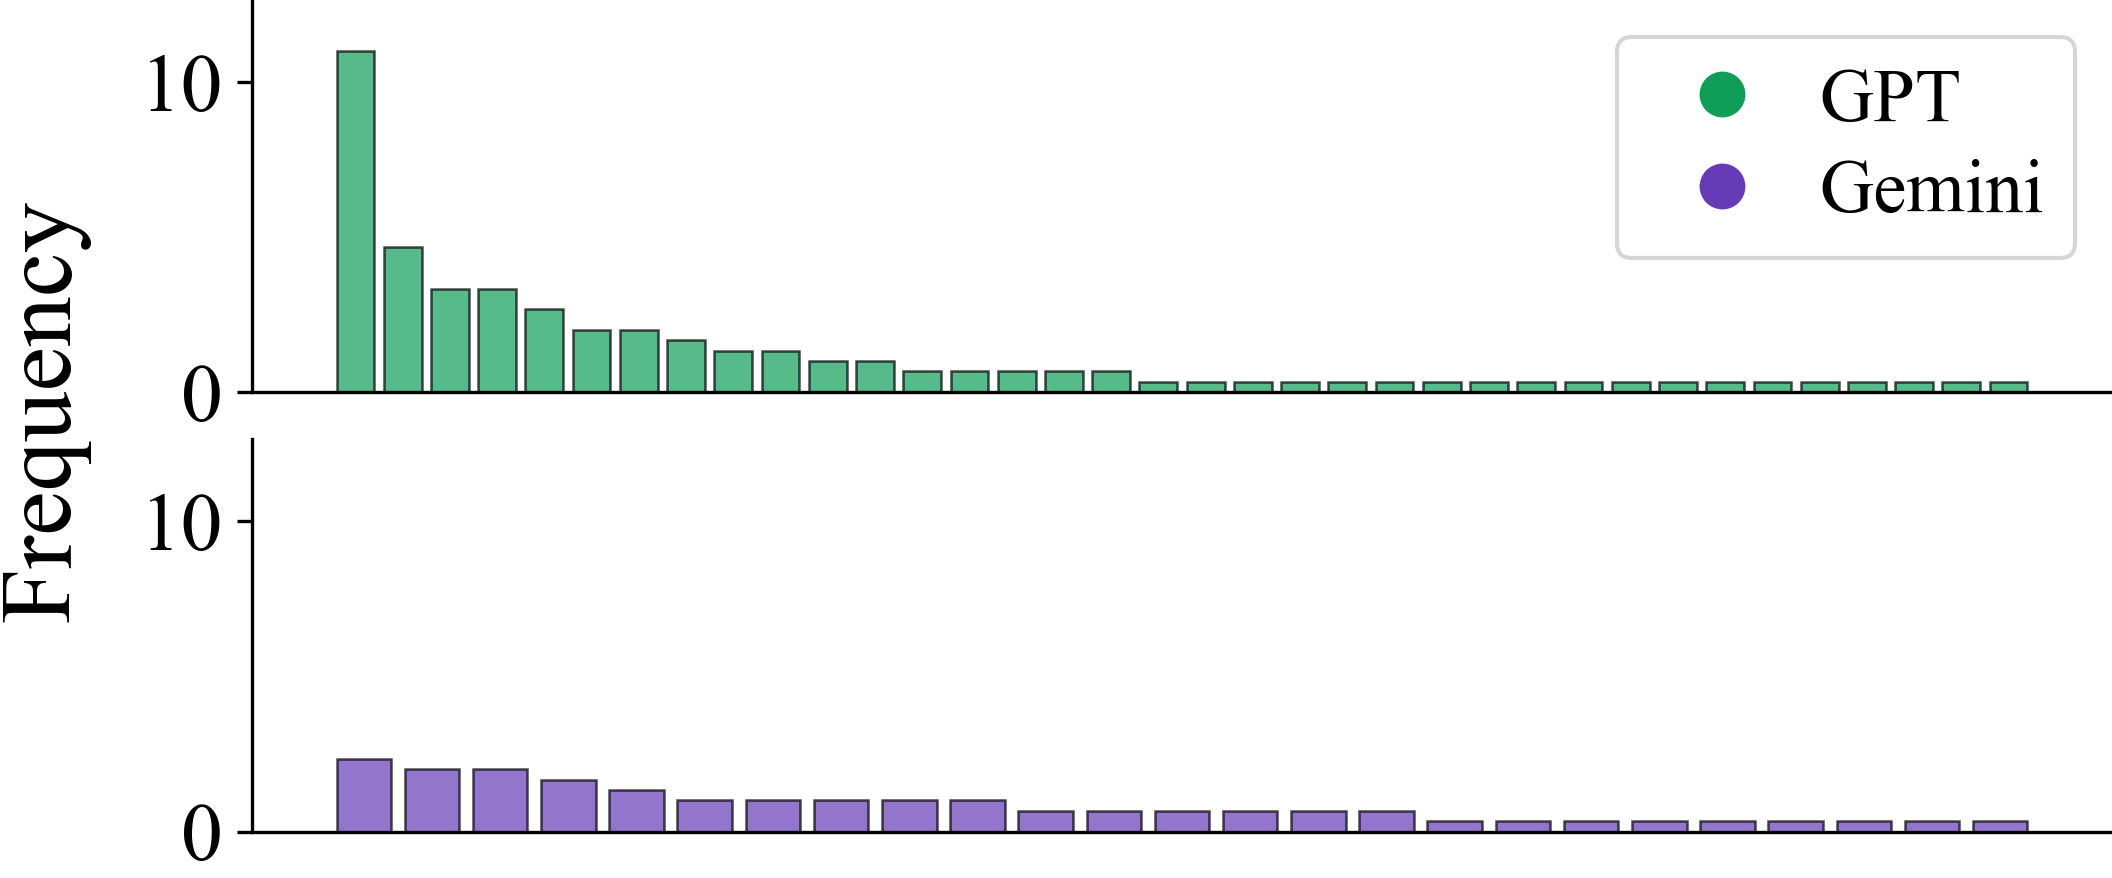
\includegraphics[width=\linewidth,height=\dimexpr\ht\transferbox+\dp\transferbox\relax,keepaspectratio]{Figure_srcs/template_frequency_gpt_vs_gem.png}
        \captionof{figure}{Per-run template citation frequency.}\label{fig:template_frequency_gpt_vs_gem}
    \end{minipage}\hfill
    \begin{minipage}[b]{0.53\linewidth}
        \centering
        \usebox{\transferbox}
        \captionof{table}{Template transferability on the Repository setting.}\label{tab:transfer}
    \end{minipage}
\end{figure*}

\paragraph{Effect of LLM-Call Budget.}
The diversity analysis explains why \textsc{Multi-Agent} stops accumulating new problems, but it leaves open whether a larger budget could close the gap.
To address this, we vary the per-instance LLM-call budget $k$ from 2 to 10, where $k$ corresponds to the iteration cutoff for \textsc{TIDE} and to the number of aggregated parallel agents for \textsc{Multi-Agent}.
As shown in Figure~\ref{fig:budget_scaling}, \textsc{TIDE} scales steeply with $k$, while \textsc{Multi-Agent} plateaus early. Interestingly, \textsc{Multi-Agent} at $k{=}10$ still falls below \textsc{TIDE} at $k{=}2$.
This suggests that the gains of iterative discovery extend beyond retrieval coverage to identification and resolution, and more fundamentally, that scaling parallel agents is no substitute for iterative conditioning.

\begin{figure}[!t]
    \centering
    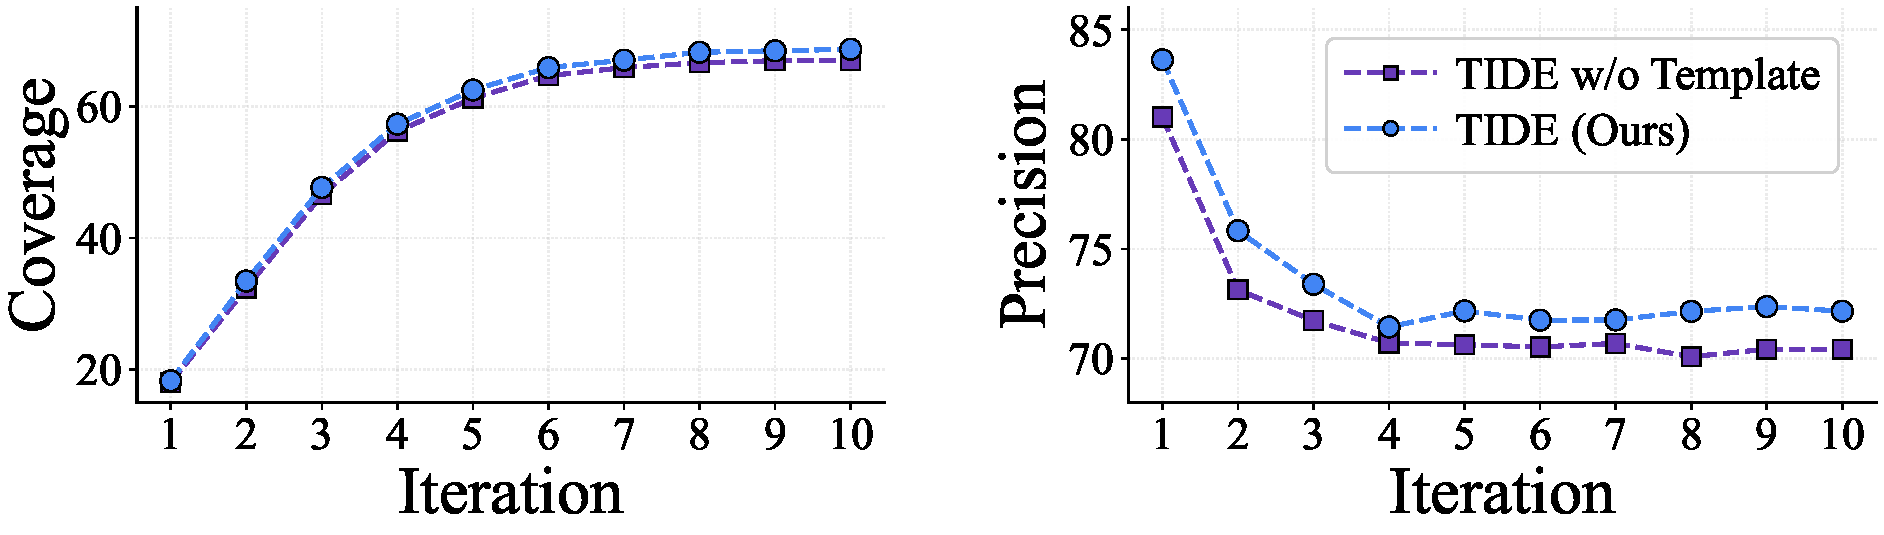
\includegraphics[width=0.975\linewidth]{Figure_srcs/iteration_recall_precision.pdf}
    \vspace{-0.075in}
    \caption{Per-iteration retrieval coverage (left) and precision (right) on the Workspace setting with GPT.}
    \label{fig:iter_recall_precision}
    \vspace{-0.05in}
\end{figure}


\paragraph{Effectiveness of Thought Templates.}
Having shown that iterative discovery enables \textsc{TIDE} to keep surfacing new problems across iterations, we now turn to what templates contribute.
To this end, we ablate templates from \textsc{TIDE} and track retrieval coverage and precision, which measure how often each predicted problem corresponds to a gold and how much of the gold pool is recovered, respectively.
Figure~\ref{fig:iter_recall_precision} shows that the template-guided variant yields a small additional coverage gain over the no-template ablation (left) and a more pronounced precision margin at every iteration (right).
This shows that iteration and templates play complementary roles: iteration mainly drives how much of the gold pool is recovered, while templates mainly drive how accurate each recovered item is.

\paragraph{Few-Shot as Template Substitute.}
We next ask whether few-shot demonstrations can replace the thought templates in \textsc{TIDE}.
To examine this, we follow the same iterative setup as \textsc{TIDE} but replace its thought templates with raw few-shot demonstrations drawn from the same training pool used to construct the templates.
As shown in Table~\ref{tab:fewshot}, demonstrations within the iterative loop fall well short of \textsc{TIDE} across retrieval, identification, and resolution.
This indicates that the value of templates lies in abstracting past examples into reusable reasoning patterns rather than in merely exposing the agent to them.

\paragraph{Template Usage Distribution Across LLMs.}
Next, we examine how each backbone draws from its own template pool during inference.
Figure~\ref{fig:template_frequency_gpt_vs_gem} shows the average per-run usage frequency of cited templates, sorted in descending order for each LLM.
GPT concentrates more sharply on a few recurring templates, whereas Gemini spreads citations more evenly across its cited pool.
These divergent usage patterns raise the question: do templates built by one backbone still transfer to another?

\paragraph{Cross-LLM Template Transferability.}
To address this, we fix the inference LLM and vary the template source between GPT and Gemini.
As shown in Table~\ref{tab:transfer}, transferred templates perform comparably to self templates across all three components and in both directions, indicating that templates remain reusable across backbones despite each LLM's distinct usage profile.

\paragraph{Effect of Template Pool Size.}
To examine how performance scales with the size of the template pool, we vary the number of available templates and report results in Figure~\ref{fig:template_count_scaling}.
Notably, iteration alone already outperforms \textsc{Single-Agent} on all three components, and adding templates yields further gains that grow with the pool size.

\begin{figure}[t]
    \centering
    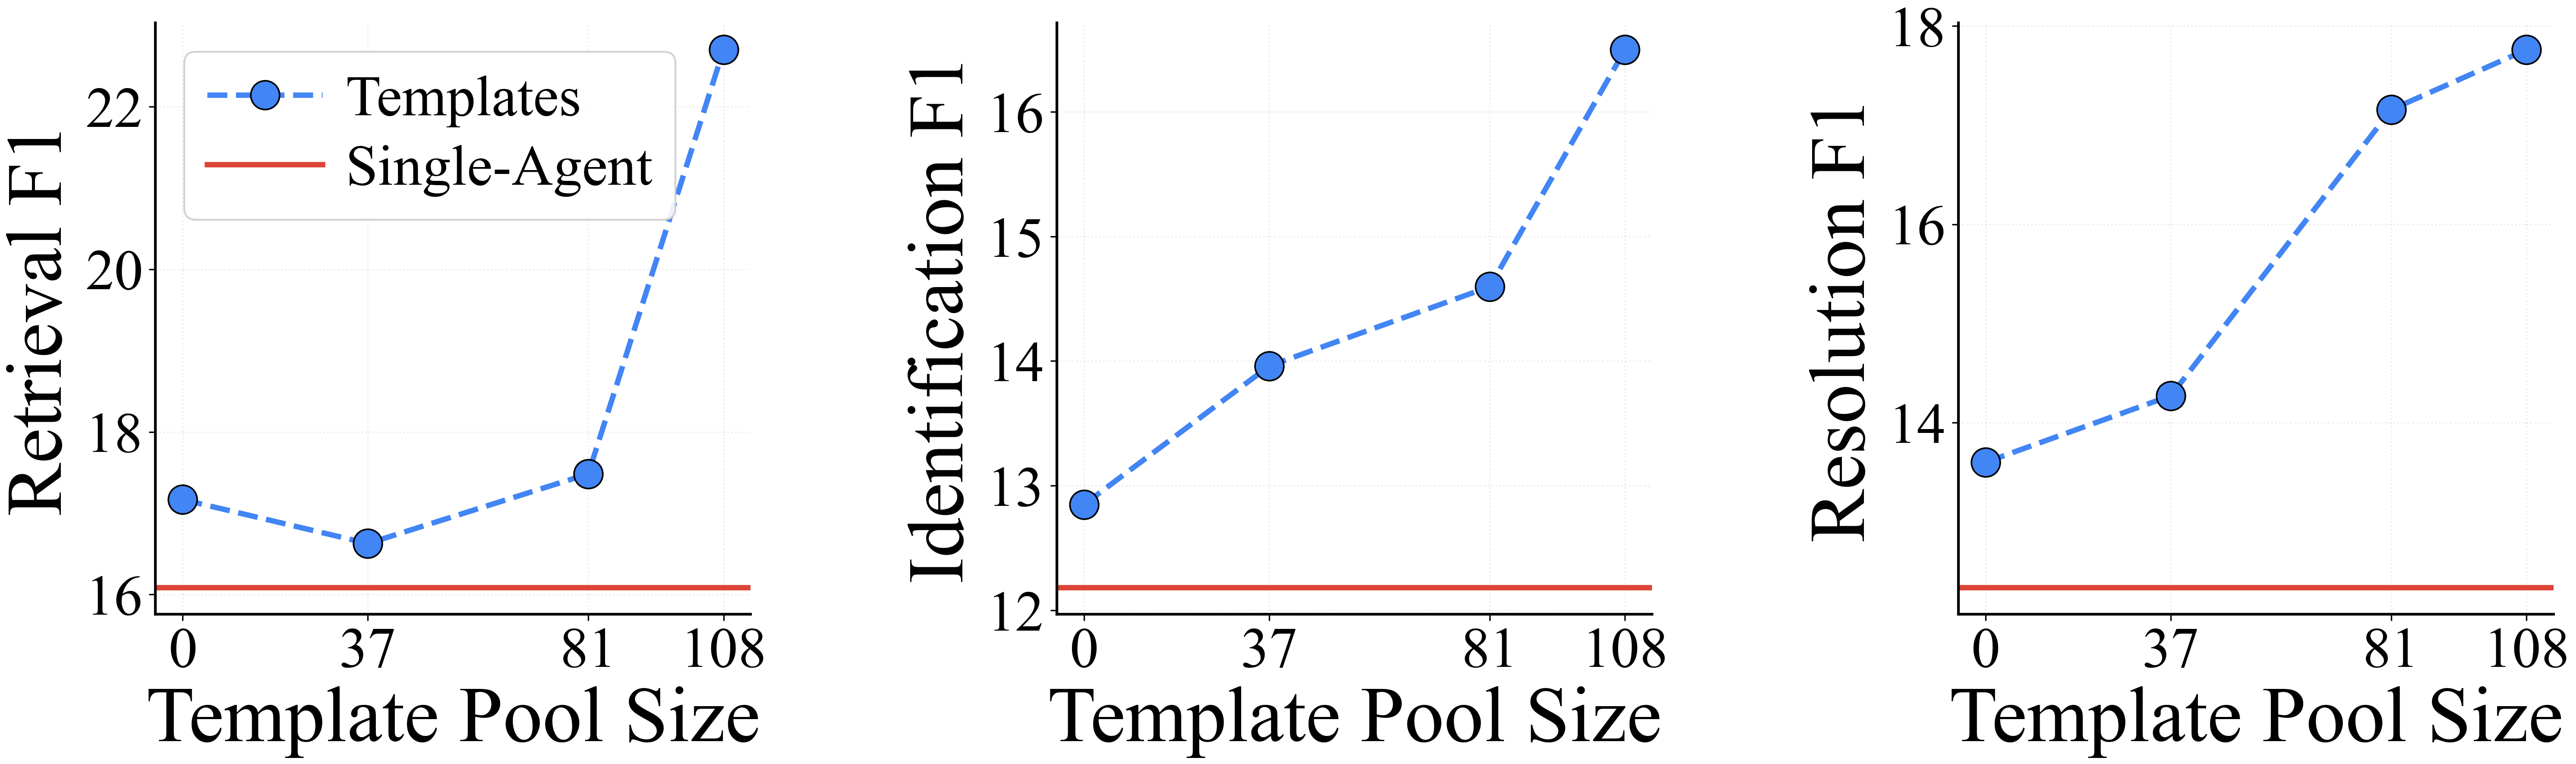
\includegraphics[width=0.975\linewidth]{Figure_srcs/template_count_scaling.png}
    \vspace{-0.075in}
    \caption{F1 scores as the template pool size grows on the repository setting with Claude.}
    \label{fig:template_count_scaling}
    \vspace{-0.1in}
\end{figure}


\subsection{Qualitative Study}
Beyond the quantitative gains shown above, we provide a qualitative analysis on two representative cases, one from each evaluation setting.
In the workspace case (Table~\ref{tab:case_study_workspace}), the gold issue is that the volunteer-tracking platform double-counts Mar 8 \textit{Community Build Day} check-ins, and the vendor patch is blocked behind a pending IT Security access approval ahead of a Mar 20 senior-leadership briefing. \textsc{Single-Agent} surfaces only an unrelated facility-rider procurement stall and retrieves none of the gold documents, so the identification, the chosen action, and the addressee are all wrong. \textsc{TIDE}, by contrast, reaches the data-integrity issue in a later iteration, retrieves the gold documents, and escalates to the right manager with the gating access ticket, the vendor-deployment deadline, and the presentation deadline.
In the repository case (Table~\ref{tab:case_study_repo}), the gold issue is a multi-function bug in \textit{mlxtend}'s \texttt{mlxtend/evaluate/mcnemar.py}: the paired helpers \texttt{mcnemar\_table} and \texttt{mcnemar\_tables} both populate the 2$\times$2 McNemar contingency table with mirrored off-diagonal assignments, so the fix has to swap \texttt{tb[1, 0]} and \texttt{tb[0, 1]} in step across both constructors. \textsc{Single-Agent} returns the two paired helpers as two isolated single-function bottlenecks, fixing each in place but never naming the shared pattern that ties them together. \textsc{TIDE}, guided by a mirrored-index-assignment template, retrieves both gold constructors inside a single bottleneck and frames the swap as one coupled defect to repair in step, recovering the multi-function fix site that the single-pass agent splits apart.
In both cases, \textsc{TIDE}'s prediction is guided by a thought template that captures a pattern recurring across instances within the same setting.
